
%!TEX ROOT=main.tex


\part{Realization}
\label{chap:realization}
Since there are no spare parts available for the transmitter or the car, all modifications have been made with as little structural intervention as possible. This process can be referred to as retrofitting.

\section{Transmitter}
\label{sec:real_tx}
\subsection{Power supply}
As described in section \ref{sub:hw_mods}, the transmitter is powered by a 2-cell LiPo battery with a nominal voltage of \SI{7.4}{\V}. The battery is connected via an XT60 connector and a switch to a step-down converter module with an LM2596 chip. The module is needed to regulate the battery voltage to \SI{5}{\V} to power the control board.

This voltage is used for the RGB LED, communication module, and linear voltage regulator AP2111, which regulates it to \SI{3.3}{\V} used to power the rest of the components. This regulator was selected because of the low dropout voltage of only \SI{250}{\mV} and high output current of \SI{600}{\mA} \cite{ap_datasheet}.		%TODO measure TX current?

In order to measure the battery voltage with the processor's internal ADC, it first had to be lowered to fit within the ADC range, which is $0\, \text{-}\, 3.3$\unit{\V}. Therefore a voltage divider is soldered to the input terminals of the step-down module. The divider was designed to use resistors with standard values and is pictured in figure \ref{fig:tx_div}. The resistor values are R1 = \SI{22}{\kohm}, R2 = \SI{10}{\kohm}.
\begin{figure}[ht]
\centering
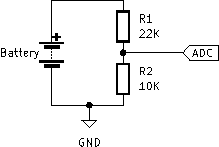
\includegraphics[width=0.4\linewidth]{fig/voltage_divider.pdf}
\caption{Voltage divider utilized in the transmitter }
\label{fig:tx_div}
\end{figure}

A fully charged 2-cell LiPo battery reaches \SI{8.4}{\V}, then the output of the divider equals
\begin{equation}
	U_{adc} = U_{batt} \cdot \frac{R2}{R1+R2} = \SI{2.625}{\V}\ ,
\end{equation}
which is safely within the ADC range.

\subsection{Controls}
The transmitter was supplied with a steering wheel and trigger as \SI{5}{\kohm} potentiometers. Since they are old, a \SI{100}{\nF} capacitor was added between the output pin of both potentiometers and ground to form a low-pass filter and smooth out the output signal.

Potentiometers used for control trimming were replaced with quadrature rotary encoders with push-buttons. Encoders have screw threads, as can be seen in figure *fig*, which fit into the original holes. Since encoders are fixed to the transmitter, a simple connector made from a pin socket was soldered to encoder pins [\todo fotka].

\subsection{PCB design}
As the space in the transmitter case was limited, it was decided not to use the perfboard but to create the PCB. It was designed in KiCad and manufactured by JLCPCB. The board consists of connectors, a voltage regulator, an MCU circuit with a crystal oscillator, and an RGB LED driven by N-channel MOSFETs. All traces are rounded to eliminate the possibility of signal reflection.

As stated in section \ref{sec:hw_control}, the prototyping was done using a BlackPill board with a microcontroller STM32F303CCT6. This microcontroller was suitable and was therefore selected also for the final design.

First, the original PCB was measured so that the new PCB could be designed according to these dimensions. A minor modification was done; the new PCB has a cutout on the top to fit the nRF24 communication module.

The communication module and control potentiometers are directly soldered to the board. In contrast, the power supply is connected via the JST XH connector, and rotary encoders are connected via simple pin sockets shown in figure *fig*.

Microcontroller circuitry was designed according to Section 7 of \cite{f3_design_an}. Four \SI{100}{\nF} ceramic decoupling capacitors were placed as close to the microcontroller as possible. Since the VBAT pin is not utilized, it was connected to the supply voltage (VDD) via another \SI{100}{\nF} ceramic capacitor. A bigger \SI{4.7}{\uF} decoupling capacitor is placed on the main supply line close to the microcontroller.

The reset circuit was also inspired by \cite{f3_design_an} and consists of a button and a capacitor connected to reduce the push-button bouncing effect. BOOT0 pin is pulled to the ground with a resistor, but switching the boot mode with a jumper placed on J1 [\todo reference] is possible.

\begin{figure}[t]
\centering

\includegraphics[width=0.55\linewidth]{fig/oscillator.pdf}
\caption{Crystal oscillator circuit}
\label{fig:osc}
\end{figure}

External \SI{12}{\MHz} crystal oscillator XT324 with a load capacitance of \SI{20}{\pF} provides the clock for the microcontroller \cite{xt324_datasheet}. The circuit of the oscillator is in figure \ref{fig:osc}. Equation \ref{eq:load_cap} mentioned in Section 3.3 of \cite{osc_design_an} was used to calculate values of external load capacitances:
\begin{equation}
C_L = \frac{C_{L1} \cdot C_{L2}}{C_{L1} + C_{L2}} + C_S\ ,
\label{eq:load_cap}
\end{equation}
where $C_L$ is the crystal's desired load capacitance, $C_{L1}$ and $C_{L2}$ are values of external capacitors and $C_S$ is the stray capacitance of the printed circuit board and connections. A rough estimate of $C_S = \SI{7}{\pF}$ according to Section 6.3.7 of \cite{f303_datasheet} and Section 3.3 of \cite{osc_design_an} was used for computation. Assuming that $C_{L1} = C_{L2}$, we have
\begin{equation}
C_L - C_S = \frac{C_{L1} \cdot C_{L1}}{C_{L1} + C_{L1}} = \frac{C_{L1}}{2} = \SI{13}{\pF}\ ,
\end{equation}
and therefore the external load capacitance should be \SI{26}{\pF}. As this is a non-standard value, \SI{27}{\pF} capacitors were used instead.

The RGB LED resistor values were chosen experimentally to achieve similar luminosity of all channels as no datasheet is available. If all channels are active, the total current through the LED does not exceed the assumed maximal \SI{20}{\mA}. [\todo fotka]


\section{Car}
\label{sec:real_car}
\subsection{Power supply}
The main power source is a 2-cell LiPo battery discussed earlier in section \ref{sec:hw_mods}, which is connected via an XT60 connector to the ESC.

Between the battery and ESC is an ACS712 current measurement module with XT60 connectors on both sides. The module is connected backward as only a positive current is measured. Consequently, the sensor output is within 0.5 to 2.5V, and ADC can safely measure it without extra components. [\todo fotka]

The control board is powered by ESC's Battery Elimination Circuit (BEC), producing \SI{5}{\V} with a maximum current of \SI{2}{\A}. Therefore ESC's power switch also acts as the main power switch. Moreover, BEC supplies power to the servo, current sensor, and, as with the transmitter, to the communication module and LEDs.

The rest of the electronics is powered by \SI{3.3}{\V} regulated by BlackPill's onboard voltage regulator. Marking on the bottom side of the board claims that the regulator can produce \SI{180}{\mA} of output current, which should be sufficient to power all the components; hence no external voltage regulator was added.

\subsection{Board design}
The Control board for the car was created on the perfboard as it allowed for more flexibility in design and testing, and the space available in the car is quite ample. The Schematic was drawn in KiCad. The board looks more complex than the board in the transmitter due to the number of components and consists of necessary connectors, a BlackPill board, an OLED display, an SD card slot, and LEDs.

The main BlackPill board is soldered directly to the perfboard to ensure rigidity. The OLED display and SD card slot were also soldered directly to the board under the BlackPill. Right under the display is a push-button used to wake it up. The UART debug pins are at the bottom left of the display, and to the right is a two-position DIP switch.

Everything not soldered to the board is connected using JST XH connectors. At first, simple pin headers were used as connectors, but the cable was sometimes disconnected from the board since the car moves and generates vibrations. JST XH connectors feature a small locking mechanism to reduce the risk of disconnection and are therefore suitable.

The board was designed so that connectors are grouped by type. In the upper left corner are the connectors for measuring the voltage, current, and temperature of the BLDC. More to the right are the connectors for the communication module, 2-pin for power, and 6-pin for SPI communication. To the right of the BlackPill board are connectors for controlling the car; closer to the board is the servo connector, and next to it is the ESC connector, which supplies voltage to the board. The last connector in the lower right corner is for the IMU. [\todo fotka]

In the right upper part of the board, there is again an RGB LED with individual channels driven by N-channel MOSFETs. The same resistor values were used since the RGB LED is the same type as the RGB LED in the transmitter. An additional wide-angle white LED controlled by a switch was mounted on the board. The purpose of this LED is to illuminate the car body, so the car is better visible at night.

As the BEC powers the control board with fixed \SI{5}{\V} output and there is no way to deduce the supply voltage without modifying the ESC, another method had to be found. LiPo batteries use the same JST XH connectors used on the control board to balance the cells when charging. Therefore the balance connector is advantageously used for battery monitoring. The user only needs to connect the battery balance connector to the appropriate socket on the board.

\subsection{Parts mounting}
The control board was fixed to the chassis simply with tape for the testing phase. As this is not ideal in the long term, it was decided to utilize the original mounting holes present in the chassis and design a frame that would fit into them to minimize drilling.

The frame design was made in \textit{Autodesk's} Fusion360 CAD software and manufactured on the 3D printer. The frame is pretty simple; it serves as an "adapter" for holes in the chassis and holes in the perfboard. The control board mounting holes are 5mm higher than the frame mounting holes to create a small gap.

There is also a mounting point for the IMU since it should be firmly attached to the chassis for correct measurements. Even though the IMU has two holes, it is mounted with only one screw. That is because the screw head in the second hole would interfere with electrical components on the IMU module.

As the mounting holes in the chassis are not at the same height, custom spacers were also designed and 3D printed to level the whole frame.
[\todo soubory, fotky]
